% 2018 全国Ⅲ卷文科/理科第23题供考生作图用的空白方格直角坐标系
% 依据源 PDF 第 2 页原图：中心在原点的 14×14 方格网（左右各 7 格、上下各 7 格），标注 O 与坐标轴上的 1。
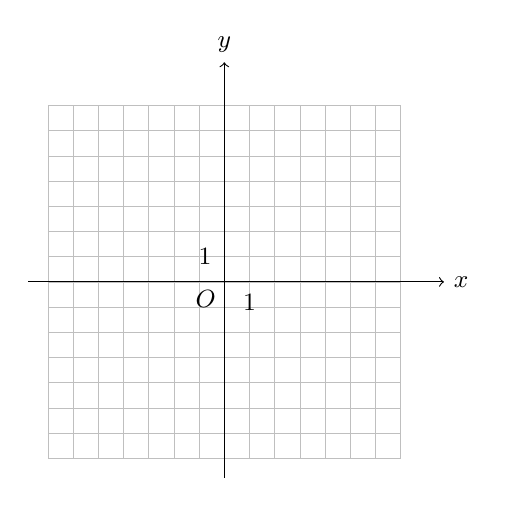
\begin{tikzpicture}[font=\small, line width=0.4pt]
  \def\u{0.32}% 单位格边长
  \pgfmathsetmacro{\xa}{-7}\pgfmathsetmacro{\xb}{7}
  \pgfmathsetmacro{\ya}{-7}\pgfmathsetmacro{\yb}{7}
  % 方格网
  \draw[gray!50, line width=0.25pt] ({\xa*\u},{\ya*\u}) grid[step=\u] ({\xb*\u},{\yb*\u});
  % 坐标轴
  \draw[->] ({\xa*\u-0.25},0) -- ({\xb*\u+0.55},0) node[anchor=west] {$x$};
  \draw[->] (0,{\ya*\u-0.25}) -- (0,{\yb*\u+0.55}) node[anchor=south] {$y$};
  % 原点与单位刻度
  \node[anchor=north east, inner sep=2pt] at (-0.03,-0.03) {$O$};
  \node[anchor=north,      inner sep=3pt] at ({1*\u},-0.05) {$1$};
  \node[anchor=east,       inner sep=3pt] at (-0.05,{1*\u}) {$1$};
\end{tikzpicture}
